\chapter{Khảo sát và các vấn đề liên quan}
\label{Chapter2}

\emph{Chương này trình bày kết quả khảo sát thực tiễn và các vấn đề liên quan để xây dựng chatbot.}

\section{Khảo sát thực trạng}
\section{Giới thiệu về chatbot}
Chatbot là một chương trình máy tính được xây dựng để có thể trò chuyện với con người. Một chat-bot đơn giản có thể dùng để thay con người trả lời các câu hỏi lặp đi lặp lại của người dùng như: “Sự kiện X diễn ra khi nào?”, “Vinaphone MAX70 là gì?”, “iPhone X giá bao nhiêu?”,… Chatbot cũng có thể đóng vai trò là một trợ lý ảo, trợ giúp trong các công việc phức tạp hơn như hỗ trợ đặt hàng, đăng ký một sự kiện, hoành thành các biểu mẫu,… hầu hết các công việc/hoặc tác vụ có thể được thực hiện theo các bước.

Ưu điểm của chatbot
\begin{enumerate}
    \item Cung cấp dịch vụ khách hàng nhanh chóng hơn:
          \begin{itemize}
              \item[--] Phần mềm này hỗ trợ doanh nghiệp cung cấp dịch vụ khách hàng 24 giờ/ngày, bất kể cuối tuần hay nghỉ lễ.
              \item[--] Khi khách hàng trực tuyến có thắc mắc, họ chỉ cần hỏi trong chatbot trên trang web của bạn mà không cần phải chờ đợi lâu để có câu trả lời. Bởi câu trả lời chỉ là một vài tổ hợp được lập trình sẵn.
          \end{itemize}
    \item Làm tăng sự hài lòng của khách hàng:
          \begin{itemize}
              \item[--] Khi khách hàng nhận được câu trả lời thỏa đáng với dịch vụ nhanh chóng nhờ chatbot, họ sẽ cảm thấy hài lòng hơn và tiếp tục mua sản phẩm của bạn.
          \end{itemize}
    \item Giảm chi phí lao động:
          \begin{itemize}
              \item[--] Chatbot giúp bạn giữ chi phí kinh doanh thấp bởi số tiền bạn đầu tư vào chatbot ít hơn số tiền bạn phải trả cho nhân viên.
              \item[--] Bằng cách này, bạn thực sự tiết kiệm được rất nhiều tiền thay vì việc duy trì một trung tâm hỗ trợ khách hàng. Tính năng này sẽ giúp bạn tiết kiệm tài chính, tránh những rắc rối trong quản lý nhân sự, và tiết kiệm thời gian để làm những việc cần thiết khác.
          \end{itemize}
    \item Nhiều mục đích sử dụng:
          \begin{itemize}
              \item[--] Bạn có thể sử dụng chatbot trong nhiều mảng, ví dụ như nhận đơn đặt hàng của khách, dịch vụ khách hàng và quảng cáo sản phẩm.
          \end{itemize}
\end{enumerate}
\begin{figure}[htp]
    \centering
    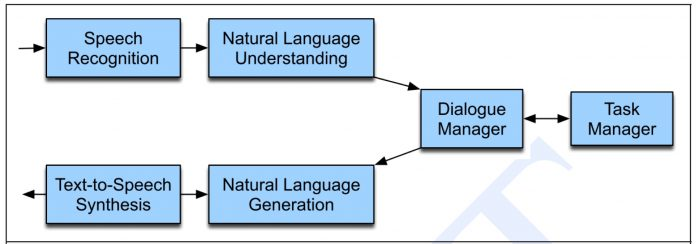
\includegraphics[width=10cm]{images/k.jpg}
    \caption{Kiến trúc cơ bản của một hệ thống giao tiếp tự động}
    \label{fig:system-class-intent}
\end{figure}

Các hệ thống chatbot giao tiếp với con người bằng giọng nói (như Siri) hoặc bằng văn bản (như các chatbot phát triển trên nền Facebook Messenger). Dù giao tiếp bằng hình thức nào, chatbot cũng cần phải hiểu văn bản để có thể đưa ra những câu trả lời phù hợp cho khách hàng. Thành phần đảm nhiệm công việc này trong hệ thống chatbot được gọi là \ac{nlu}, trong đó có rất nhiều các kỹ thuật xử lý ngôn ngữ tự nhiên (\ac{nlp}) được áp dụng.
\\
Hai thành phần liên quan đến xử lý ngôn ngữ tự nhiên không thể thiếu của một \ac{nlu} module là bộ phân loại ý định và nhận diện thực thể (NER). Phân loại ý định giúp chat-bot hiểu ý định của người dùng. Về mặt bản chất phân loại ý định chính là một bài toán phân loại câu với tập nhãn là các ý định có thể có của người dùng (đã được định nghĩa từ trước). NER giúp chat-bot trích xuất các thông tin trong yêu cầu/câu trả lời của người dùng. Các thông tin đó có thể là tên sản phẩm, địa chỉ, số điện thoại, số tài khoản của người dùng,… NER là một bài toán gán nhãn chuỗi cơ bản: cho vào một câu đầu vào, trích xuất tất cả các thực thể định danh trong câu và phân loại chúng vào một trong các nhãn đã được định nghĩa từ trước.
\\
Một thành phần xử lý ngôn ngữ tự nhiên khác có thể được thêm vào chat-bot là bộ quản lý hội thoại, bộ sinh ngôn ngữ (NLG), và bộ phân tích cảm xúc. Một bộ quản lý hội thoại sẽ lưu trữ, phân tích và tận dụng ngữ cảnh cuộc hội thoại và giúp chat-bot suy luận hành động tiếp theo trong khi NLG giúp sinh câu trả lời đầy đủ, tự nhiên nhất bằng ngôn ngữ tự nhiên cho chat-bot. Một bộ phân tích cảm xúc có thể cần bởi vì cùng một câu có thể mang nhiều nghĩa khác nhau trong các văn cảnh khác nhau, do đó có thể cần được trả lời theo các cách khác nhau phụ thuộc vào cảm xúc của người dùng.
\\
Bài luận này chủ yếu nghiên cứu về phát hiện ý định và trích xuất thực thể trong NLU module.

% \subsection{Một số phương pháp hiểu ngôn ngữ tự nhiên}

% \begin{itemize}
%     \item Rasa \ac{nlu}
%           \begin{figure}[htp]
%               \centering
%               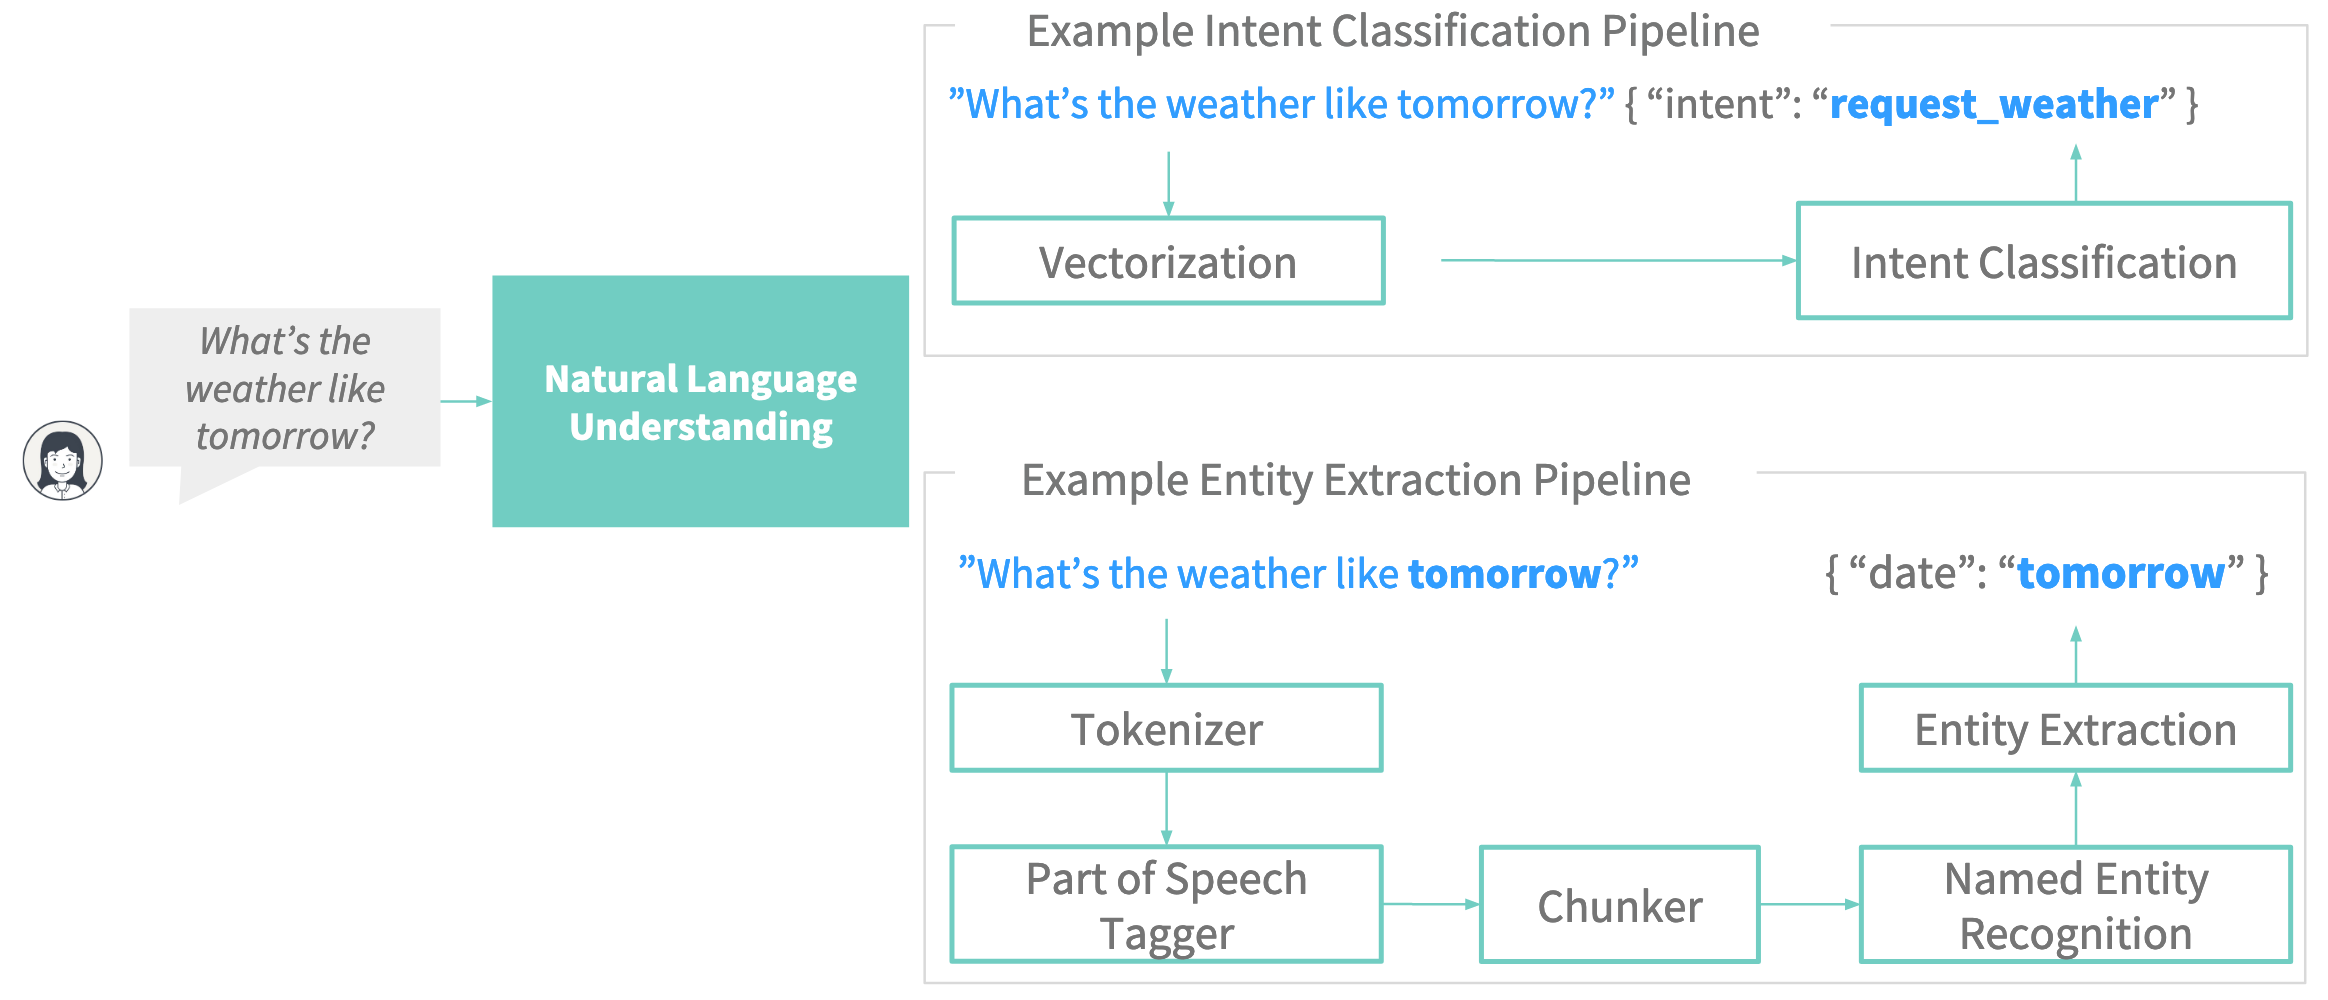
\includegraphics[width=10cm]{images/Rasa-NLU.png}
%               \caption{Sơ đồ hệ thống Rasa-\ac{nlu}}
%               \label{fig:rasa-nlu}
%           \end{figure}
%     \item Snips \ac{nlu}
%           \begin{figure}[htp]
%               \centering
%               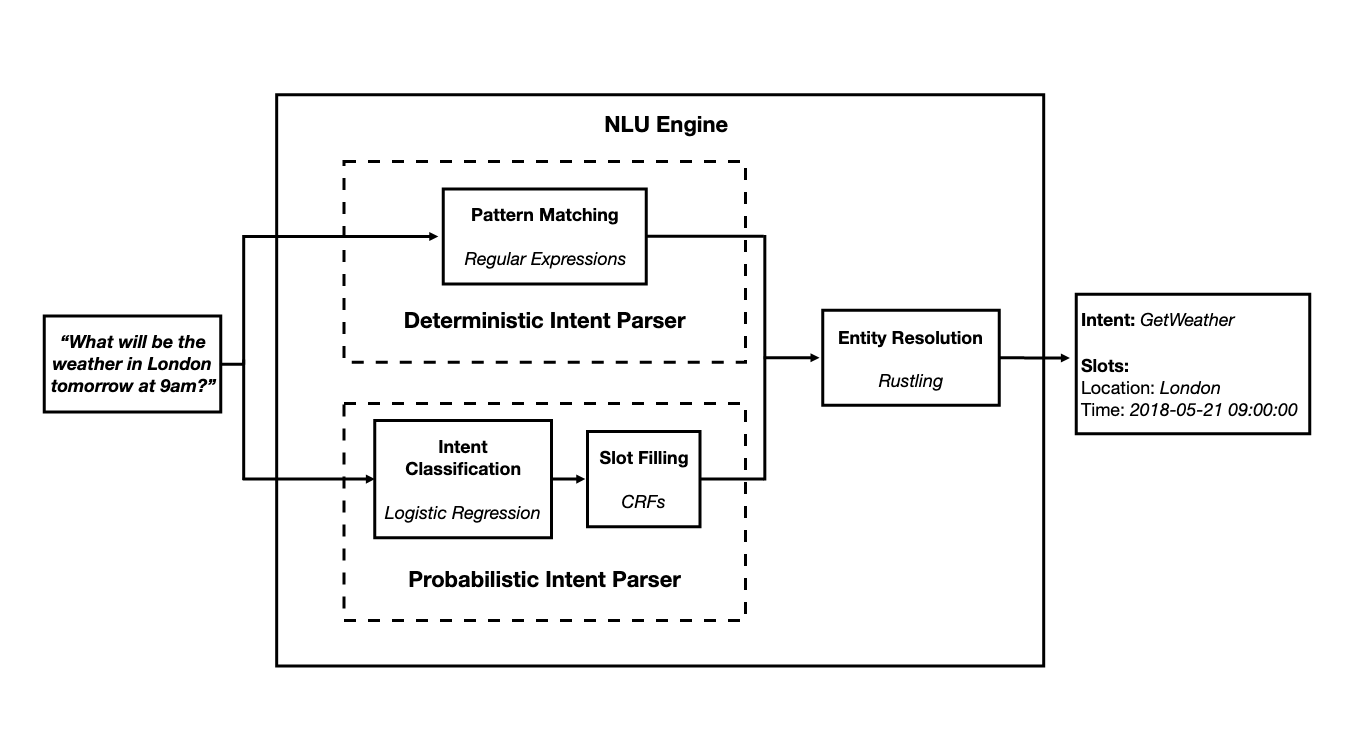
\includegraphics[width=10cm]{images/Snips-NLU.png}
%               \caption{Sơ đồ hệ thống Snips-\ac{nlu}}
%               \label{fig:snips-nlu}
%           \end{figure}
%           Có thể khái quát các luồng xử lý của snips-NLU \cite{snips-nlu} như sau:
%           Hệ thống Snips-NLU (hình \ref{fig:snips-nlu}) chứa một thành phần chính, NLU Engine, bản thân nó bao gồm một số thành phần sau:
%           \begin{itemize}
%               \item Deterministic intent parser: Mục tiêu của trình phân tích cú pháp xác định là cung cấp độ mạnh mẽ và trải nghiệm có thể dự đoán được cho người dùng vì nó được đảm bảo đạt được 1.0 F1-Score trên các ví dụ đào tạo. Các truy vấn có trong dữ liệu huấn luyện được sử dụng để xây dựng các mẫu bao gồm tất cả các tổ hợp giá trị thực thể.
%               \item Probabilistic intent parser: Trình phân tích cú pháp mục đích nhằm mục đích mở rộng phân tích cú pháp vượt ra ngoài các ví dụ đào tạo và nhận ra các biến thể không xuất hiện trong dữ liệu đào tạo. Nó cung cấp sức mạnh tổng quát hóa mà trình phân tích cú pháp xác định thiếu. Thông qua hai bước intent classification (xác định ý định) and slot filling (trích xuất thực thể).
%               \item Entity resolution:
%           \end{itemize}
% \end{itemize}
